% file: tournament.tex

\documentclass{standalone}
\usepackage{tikz}
\usepackage{tikz-qtree}
\usetikzlibrary{shapes}

\newcommand{\red}[1]{\textcolor{red}{#1}}

\begin{document}
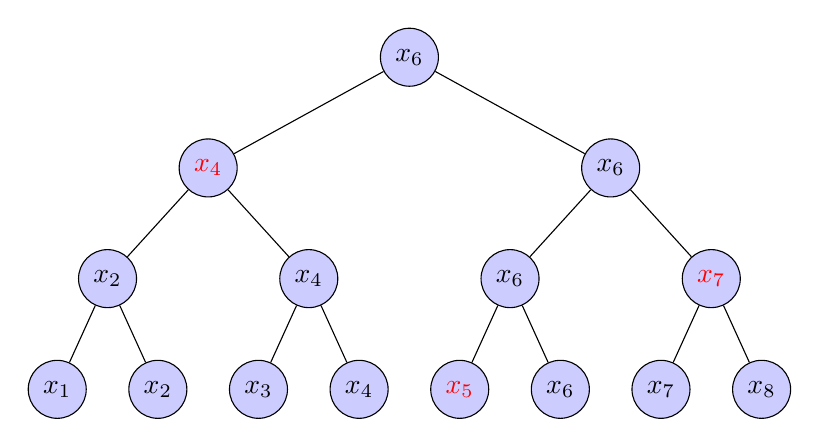
\begin{tikzpicture}[level distance = 40pt, sibling distance = 15pt,
  edge from parent/.style= { % added code
      draw, edge from parent path = {(\tikzparentnode) -- (\tikzchildnode)}},
    leaf/.style = {rectangle, rounded corners, fill = lightgray!40}]
  \tikzset{every tree node/.style = 
    {align = center, circle, draw, fill = blue!20}}

    \Tree [.{$x_6$}	
	    [.\red{{$x_4$}}
	       [.{$x_2$}
		 [.{$x_1$} ]
		 [.{$x_2$} ]
	       ] 
	       [.{$x_4$} 
		 [.{$x_3$} ]
		 [.{$x_4$} ]
	       ]
            ]
	    [.{$x_6$} 
	      [.{$x_6$} 
		[.\red{{$x_5$}} ] 
		[.{$x_6$} ] 
	      ] 
	      [.{\red{$x_7$}} 
		[.{$x_7$} ] 
		[.{$x_8$} ] 
	      ]
	   ] 
        ]
  \end{tikzpicture}
\end{document}
